\documentclass[../access.tex]{subfiles}
\graphicspath{{\subfix{../Images}}}

\begin{document}
    \subsection {Cryptographic Tools in Literature}
        \label{cryptographic-methods}
        \subsubsection{Threshold Systems}
            \label{threshold_systems}            
            Threshold systems were developed to add redundancy to the sharing of secret information. Adi Shamir introduced the concept in 1979 \cite{Shamir1979} and since then it has been used in many e-voting system proposals. In \textit{threshold systems}, a piece of encrypted data \textit{D} that has been split into \textit{n} pieces or shards, i.e.,
            
            \begin{equation}
            D = D_{1}, D_{2},..., D_{n}
            \end{equation}
            
            can be reconstructed as long as \textit{k}, $ 1 \leq k \leq n $ shards are known. As long as only $ k - 1 $ pieces are known, recovering \textit{D} is theoretically possible but computationally infeasible. But as long as \textit{k} or more shards are known, recovering \textit{D} is a trivial operation \cite{Benaloh1986b}.
            A system with these properties is classified as a \textit{(k, n) threshold system}.
        
            \paragraph{Homomorphic (k, n) Threshold Cryptosystems}
                Threshold systems define two operational domains: \textit{P}, the plaintext domain and \textit{C}, the ciphertext domain. A message \textit{M} written in human-readable format belongs to domain \textit{P}, but it is possible to switch between these domains using the encryption function \textit{E} to transverse from \textit{P} to \textit{C} and the corresponding decryption function \textit{D} to move from \textit{C} to \textit{P}.
                \par
                Formally, it means that 
                
                \begin{equation}
                    E(M) = M'
                \end{equation}
                
                and
                
                \begin{equation}
                    D(M') = M 
                \end{equation}
                
                where \textit{M'} is the message in the ciphertext domain.
                \par
                Binary operations can also be defined within these domains, such as addition, subtraction, multiplication, exponentiation, etc. To differentiate between which operation is used in which domain, the symbol $ \oplus $ denotes an operation in the \textit{P} domain, whereas $ \otimes $ the respective operation when in the \textit{C} domain \cite{Benaloh1986b} \cite{Rjaskova2002}.
                \par
                Consider a secret \textit{s} belonging to the \textit{P} domain that was split into \textit{k} parts such that 

                \begin{equation}
                    s = F(t_{i1}, t_{i2}, ..., t_{ik})
                \end{equation}
                
                where \textit{F} is a cryptographic function used to switch between domains, such as the encryption and decryption functions, i.e., $ F, F \in \{C, D\} $.
                \par
                Now consider another secret \textit{s'} that was also split into \textit{k} pieces by the same function \textit{F}: 
                
                \begin{equation}
                    s' = F(t'_{i1}, t'_{i2}, ..., t'_{ik})
                \end{equation}
                
                This encryption scheme is $ (\oplus, \otimes) - homomorphic $ if:
                
                \begin{equation}
                    s \oplus s' = F(t_{i1} \otimes t'_{i1}, t_{i2} \otimes t'_{i2}, ..., t_{ik} \otimes t'_{ik}) 
                \end{equation}
                
                i.e., \textit{the composition of the shares of the secrets are shares of the composition of the secrets} \cite{Benaloh1987}.
                \par
                A practical consequence of this property is the ability to perform arithmetic operations directly on the \textit{C} domain using the homomorphic equivalent operation from the plaintext \textit{P} domain. The result of such an operation can then be decrypted, thus obtaining the plaintext equivalent.
                Consider Fig. \ref{fig:homomorphism} as an example:

                \begin{figure}[h!]
                    \centering
                    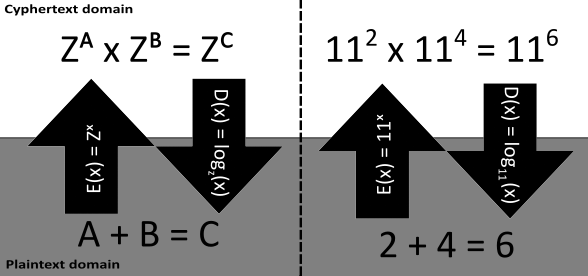
\includegraphics[width=\columnwidth]{Images/almei2.png}
                    \caption{Example of a simple homomorphic threshold system.}
                    \label{fig:homomorphism}
                \end{figure}

                In this example, data transverses to the cyphertext domain by elevating a fixed base \textit{Z} to the power defined by the data itself. The encryption is defined by the function: 
                
                \begin{equation}
                    F = E(x) = Z^x.
                \end{equation} 
                
                Information can move to the plaintext domain by applying the inverse operation, i.e., the natural logarithm of the same base \textit{Z}: 
                
                \begin{equation}
                    F' = D(x) = \log_Z(x).
                \end{equation} 
                
                We can verify this with the numerical example on the right side of Fig. \ref{fig:homomorphism}. The example shows that an addition, the $\oplus$ operator, in the plaintext \textit{P} domain is homomorphic equivalent to a multiplication, the $\otimes$ operator, in the ciphertext \textit{C} domain.

        \subsubsection{Mix-Nets}
            \label{centralized_mix_nets}
            Mix-nets take advantage of a property of asymmetrical cryptosystems: \textit{when data is encrypted and decrypted using multiple pairs of encryption keys, including re-encryptions using the same key, the order in which the respective decryption keys are applied to retrieve the original plaintext is irrelevant as long as the same number and type of keys are respected} \cite{Juels2010} \cite{Chaum1982}.
            \par
            Consider a finite set of \textit{N} public encryption keys: 

            \begin{equation}
                E_{set} = [E_{1}, E_{2}, ..., E_{N}]
            \end{equation}
            
            and the corresponding set of decryption keys: 
            
            \begin{equation}
                D_{set} = [D_{1}, D_{2}, ..., D_{N}]
            \end{equation}    
                
            Key pairs are defined by: 
            
            \begin{equation}
                (E_{1}, D_{1}), (E_{2}, D_{2}), ..., (E_{N}, D_{N})
            \end{equation}
            
            Note that $ E_{set} $ and $ D_{set} $ have the same number of elements.
            Now consider a message \textit{M} encrypted by the set of encryption keys sequentially. For simplicity’s sake, assume that these keys are applied in order: 

            \begin{equation}
                M^{e_{set}} = E_{1}(E_{2}(... E_{N}(M)))
            \end{equation}
            
            \textit{M} can be recovered using any permutation from the respective decryption key set $ D_{set} $ as long as both sets match in the number of elements and the number of applications of each key is respected:
            
            \begin{equation}
                \begin{aligned}
                    M   &= D_{1}(D_{2}(...D_{N}(M^{e_{set}}))) \\ 
                        &= D_{3}(D_{1}(D_{N}(...D_{8}(M^{e_{set}}))))\\ 
                        &= ... \\
                        &= D_{N}(...(D_{2}(D_{1}(M^{e_{set}}))))
                \end{aligned}
            \end{equation}
            
            which is valid for any permutations of $ D_{set}. $
            \par
            A mix-net protects information by applying multiple levels of encryption by applying multiple keys to it and explores the fact that, to recover the initial message, the corresponding decrypting keys need to be used but only the same number of times in which the asymmetrical counterpart was used. The order in which the decryption key set is applied is irrelevant in this case.
            \par
            If only one encryption key pair is used, the ciphertext can be attacked by providing a piece of plaintext data chosen to reveal statistical or language-specific characteristics of the encryption process \cite{Schneider1994}. Employing a mix-net does not eliminate this threat completely, but it does weaken it substantially.
            \par
            Fig. \ref{fig:mix-nets} exemplifies this process. Messages \emph{A to D} were encrypted with a series of encryption keys from asymmetrical pairs. Each message has, effectively, \emph{N} encryption layers applied to it. Each server in the mixed network contains only one of the decryption keys from the set applied before; thus, it removes only the encryption that fits that key. As long as the encrypted messages are routed through the servers that can remove all encryption layers, i.e., a set of servers that have the complete set of corresponding decryption keys used in the initial encryption, at the end of this routing process, we have the original messages.
            
            \begin{figure}[ht!]
                \centering
                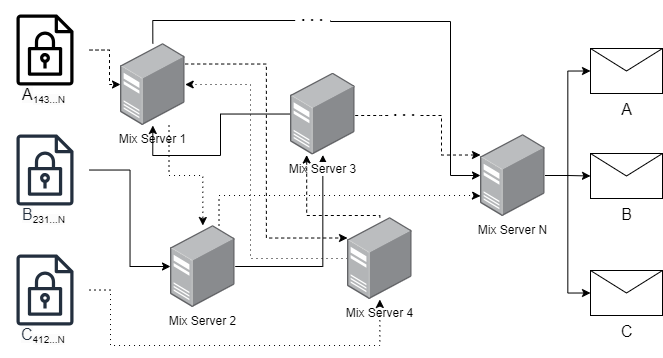
\includegraphics[width=\columnwidth]{Images/almei3.png}
                \caption{Mix Net scheme.}
                \label{fig:mix-nets}
            \end{figure}
            
            Data to mix is previously encrypted according to a secret permutation of keys in $ E_{set} $, with that permutation transmitted to all servers in the network. Each server in the mix-net network removes one layer of encryption at a time since each server stores only one decryption key. The trajectory of the encrypted data in the Mix-net network is determined by the permutation applied during the initial encryption. As long as the number and types of encryption keys are respected, the output on the last server produces the data in plaintext format.
        
        \subsubsection{Blind Signatures}
            \label{blind-signature}
            This cryptographic method was introduced in \cite{Chaum1982} in 1982 as a method to implement untraceable electronic payments. This method relies on a trusted party or element to validate a digital signature without seeing the contents of what was signed, hence the \textit{blind} adjective. This method emulates what already happens with some vote-by-mail procedures, where eligible voters receive at home a ballot \textit{blindly signed} by a trusted authority.
            \par
            As in the original article \cite{Chaum1982}, we are going to use an election example to illustrate this protocol.
            \par
            Consider two actors in an exercise: a voter that wishes to validate a voting ballot \textit{M} and a trustee that can validate messages. The trustee creates a pair of asymmetrical encryption keys, keeps the private key \textit{D} secret, and publicises the public one \textit{E}. The voter fills out his or her ballot, \textit{M}, but it needs the trustee's signature. To get it without revealing its contents, the voter follows these steps:
            \begin{enumerate}
                \item The voter begins by selecting a random number \textit{K} and keeps it secret.
                \item The voter encrypts the random number using the trustee's public encryption key: 
                    
                    \begin{equation}
                        E(K) = K^{e}
                    \end{equation}
                    
                \item The voter proceeds to blind the filled-out ballot \textit{M} by applying the previous factor to it, which in this case consists of:

                    \begin{equation}
                        B = M \cdot K^{e}
                    \end{equation}

                The blinding process is the binary multiplication of the message contents to be signed by the encrypted random number \textit{K}, and \textit{B} is the blinded message or ballot.
                \item The voter provides \textit{B} to the trustee to be signed. The trustee digitally signs \textit{B} by encrypting it with its private key \textit{D}, which actually corresponds to a decryption operation in this asymmetrical context:
                    
                    \begin{equation}
                        D(B) = B^{d} = (M \cdot K^{e})^{d} = M^{d} \cdot K^{ed}
                    \end{equation}    
                
                where 
                    \begin{equation}
                        K^{ed} = D(E(K)) = K
                    \end{equation}
                    
                and thus 
                    \begin{equation}
                        B^{d} = M^{d} \cdot K
                    \end{equation}
                    
                By multiplying the message by a factor only known to the voter, this effectively prevents the trustee from ever recovering \textit{M} without knowing \textit{K}.
                \item The trustee returns the signed blinded message $ B^{d} $ to the voter, and he/she can easily recover a signed \textit{M} by computing: 
                
                    \begin{equation}
                       \frac{B^{d}}{K} = \frac{M^{d} \cdot K}{K} = M^{d} 
                    \end{equation}
                
                since \textit{K} is only known to the voter.
            \end{enumerate}
        
            Blind signatures provide decoupling between the information to be certified and the certification process itself. Using this method, it is possible to validate election ballots and other data without needing to reveal its contents, thus preserving voter privacy while adding an important layer of security to the process.
        
        \subsubsection{Cryptographic Proofs}
            Cryptographic proofs are protocols detailing a series of steps that must be executed between two parties - a \textit{prover} and \textit{verifier} - such that the \textit{prover} can show the knowledge of a \textit{claim} to the \textit{verifier}.
            Digital signatures are good examples of cryptographic proofs: signatures are valid if the signed message is obtained after decrypting the signature with the public encryption key. This implicitly proves that the signer owns, or at least knows, the private encryption key in question.
            \par
            Cryptographic proofs can be \textit{interactive} or \textit{non-interactive} depending on the required exchanges between the \textit{prover} and \textit{verifier}.

            \paragraph{zk-SNARKs Proofs}
                Proofs that are executed without revealing any knowledge about the claim are classified as \textit{Zero-knowledge proofs (ZKP)} and are extensively used in the e-voting context. From among the types of ZKP identified in the literature, the most frequent one observed is the \textit{Zero-Knowledge Succinct Non-Interactive Argument of Knowledge (zk-SNARK)} proof. As the name implies, it is a type of \textit{non-interactive} cryptographic proof, and its popularity in the e-voting context warrants a detailed explanation of it.
                \par
                \textit{ZkSNARKs} proofs are introduced in \cite{Gennaro2013}; maturated by \cite{Parno2016}; and employed formally in \cite{Ben-Sasson2014a}. These proofs consist of a set of verifiable computation schemes with the following properties:
                \begin{itemize}
                    \item{Proofs are short and non-interactive, i.e., a verifier can be convinced with a single message from a prover.}
                    \item{Private information can be used by the prover during the generation of the proof without the verifier learning anything about that information.}
                    \item{The cost of verifying a proof is independent of the computational complexity of the input.}
                \end{itemize} 
                
                The \textit{zkSNARKs} verification scheme is based on a polynomial-based abstraction called Quadratic Arithmetic Programmes (QAPs). QAPs are obtained using two higher-level abstractions to specify arithmetic and rank-1 constraint systems (R1CS), which are needed to verify the proof. Arithmetic circuits are obtained by flattening the compiled high-level code defining the proof. This flattening operation consists of converting complex mathematical operations (exponentiations, roots, logarithms, etc.) to simpler algebraic operations, namely additions, subtractions, multiplications, and divisions. The flattened code is then converted into algebraic gates, which are then transformed into a R1CS. These can then be interpolated (using the Lagrange interpolation formula, for example) to find the QAPs that allow the original proof to be verified \cite{Eberhardt2018} \cite{Maesa2023}.

        
        \subsubsection{Additional Tools: Public Bulletin Board and Anonymous Communication Channel}
            The public bulletin board and anonymous communication channels are tools that normally pair up in the literature due to their complementary nature and usage, thus being set in the same category. They relate to the tools presented due to their use in the e-voting context and, because these are used to propagate information within the system, can have it encrypted for safety, though they do not present any new cryptographic ideas in themselves.
            \par
            The \textit{Public Bulletin Board} is an abstraction of a communication channel that can be accessed by anyone, but data can only be appended in a controllable fashion, i.e., anyone can read the append-only board, i.e., deletions are not possible, but only a few authorised entities can add new data to it. Some authors base their solution on the assumption that such a channel exists, or at least is conceivable, but not many went to the extent of providing details of a practical implementation \cite{Juels2010}.
            \par
            The \textit{Anonymous Communication Channel} is similar in terms of access control, but this one adds the property that all communications are done via pseudonyms, as well as protecting data during transmission using encryption, thus adding anonymity to the previous concept \cite{Park1994}.

    \subsection{Blockchain Background}
        A blockchain is a distributed data structure replicated through all the active nodes in a \textit{peer-to-peer (P2P)} network. New data can only be added in the form of a new block on the chain. Due to the decentralised manner in which data is distributed through the network, operations on it, namely appending new data, are regulated by a network-wide protocol that establishes the rules that must be followed by a node that pretends to add new data to it. In a blockchain, data is accessible to anyone, but deletions and modifications are not even available in the protocol.
        \par
        This protocol regulates not just the addition of new blocks to the existing chain but also ensures that only one version of the data structure exists at all active nodes through periodic synchronisation actions. This removes any sort of centralised control over this structure, thus establishing a decentralised management structure that is able to ensure the correct functioning as well as the integrity of the data in the structure without requiring any administrators or nodes with special permissions.
        \par
        Many blockchains available publicly were engineered and configured to support cryptocurrencies. As such, most of the data in these blockchains is transactional data indicating the exchange of a cryptocurrency between two addresses. All these concepts are going to be explained in greater detail, but for now, it suffices to say that these characteristics give all blockchains a set of built-in features, with \textit{immutability}, \textit{pseudo-anonymity}, and \textit{verifiability} among the ones that are more relevant in an electronic voting context.
    
    \subsubsection{Blockchain Mechanics and Consensus Protocol}
        \label{mining-consensus}
        New data is added to the blockchain in the form of a \textit{block}, which is, in its essence, a file filled with transactional data. For cryptocurrency-based blockchains, the transactions in a block that is about to be added to the top of the chain are waiting for confirmation, and it is the addition of that block to the chain that confirms a transaction. An active node in a blockchain network is a computational unit that keeps a full and synchronised copy of the blockchain in its permanent storage and can also \textit{"mine"} for new blocks.
        \par
        Though paradoxically distributed, a new block is appended to the chain with the authorization of the governing protocol. This append extends the official state of the blockchain, also updated by the remaining nodes. The consensus protocol decides which of the active nodes appends the new block. Section \ref{blockchain-consensus-protocols} details some popular choices of consensus protocols developed and implemented in public blockchains since the inception of this technology. In blockchains that support cryptocurrencies, the node that appends a new block typically gets rewarded with newly minted tokens from the supported cryptocurrency, a method that is popular among these blockchains to increase their total supply of tokens gradually and to provide an incentive for active participation in the network.
    
        \paragraph{Popular Blockchain Consensus Protocols}
        \label{blockchain-consensus-protocols}
            Blockchain consensus protocols are a dynamic area of research among blockchain enthusiasts. As such, new protocols are being conceived and implemented at a fairly high rate, which makes it difficult to completely characterise the landscape. This section aims at introducing and briefly explaining the most popular protocols among existing blockchain solutions.
                \begin{itemize}
                    \item {Proof-of-Work (PoW) - The original consensus protocol in earlier blockchains, such as Bitcoin and Ethereum version 1.0. This protocol establishes race conditions between nodes by rewarding the first node that solves a computationally intensive cryptographic puzzle. To solve this puzzle, nodes need to find the hash digest fitting a predetermined format, and nodes are limited to brute force approaches to tackle this problem. This protocol is responsible for significant energy waste since all hash computations for losing nodes are simply discarded \cite{Narayanan2016}.}

                    \item {Proof-of-Stake (PoS) - This protocol was created as an alternative to PoW once this one became problematic due to its high energy expenditure. In a PoS, nodes increase their probability of selection by the protocol by increasing their stake in the network, namely, by holding tokens of that blockchain in their accounts. The bigger the stake, the higher is the probability of them being selected to add the next block and receiving the associated block reward \cite{Bouraga2021}. Ethereum's version 2.0 upgraded the consensus algorithm from PoW to PoS.}

                    \item {Delegated Proof of Stake (DPoS) - This version of the previous protocol uses the same stake principle, but, in this case, it is used to gain voting power, which is then used to elect block verifiers, the ones that actually create new blocks. So nodes actually delegate the power they have due to their stake in the network, hence the name \cite{Zhang2020a}.}

                    \item {Practical Byzantine Fault Tolerance (PBFT)} - In this protocol, a node submits a block proposal to a principal node, which effectively acts as a network administrator, which then propagates it to multiple other backups. If enough backup nodes agree on the proposed block, it gets added to the chain. Otherwise, it is discarded \cite{Xiao2020}.
                \end{itemize}
            
                These four protocols were among the first to be suggested and are now considered core protocols from which others are derived \cite{Zhang2020a}. As the application range of blockchain solutions increased, so did the consensus protocols that supported them: applications used for medical decisions use a PoS-based protocol, aptly named \textit{Proof-of-Disease} \cite{Patel2019}. \textit{Proof-of-Elapsed-Time} is a PoW replacing consensus where nodes have to wait a period of time generated in a trusted execution environment \cite{Bowman2021} instead of solving cryptographic puzzles. \textit{Proof-of-Luck} consensus is based in PoW and PoS, but also the Proof-of-Elapsed-Time just referred, which creates an energy efficient and low latency for transaction validation consensus protocol \cite{Milutinovic2016}. In \textit{Proof-of-Authority}, an easily scalable, reputation-based protocol, validator nodes are incentivized to maintain their position (the authority) by refraining from dishonest behaviour that could warrant them a negative reputation. This is the protocol of choice of private permissioned blockchain frameworks such as the ones from the Hyperledger family, along with the \textit{Practical Byzantine Fault Tolerance} \cite{Joshi2021}. \cite{Bouraga2021}, \cite{Zhang2020a}, and \cite{Xiao2020} for more comprehensive surveys on this topic.

        \paragraph{Transactional Metadata}
        \label{transactional_metadata}
            Before Ethereum increased considerably the scope of applications that could be supported by a blockchain, any attempt to use existing blockchains (whose options were realistically reduced to Bitcoin) for any purposes other than transacting cryptocurrencies required creative ways to use the meagre set of options made available by this blockchain. Among the most popular ones was the usage of Bitcoin's \textit{OP\_RETURN} instruction, which allowed adding custom data, i.e., non-transactional data, to the information pertaining to a transaction.
            \par
            Older, Bitcoin-based decentralised proposals analysed in this exercise use this instruction, hence the importance of clarifying how it works.
            
        \paragraph{Bitcoin OP\_RETURN Instruction}
            Before \textit{OP\_RETURN}, developers were already experimenting with adding custom text to a block, and they first used \textit{Pay-to-PubkeyHash}, a standard Bitcoin script used to implement signature verification. Without getting into much detail, this script expects a hash digest as one of its inputs, and it writes it in the transaction output, specifically in the \textit{out-script} portion of the transactional data, along with the boolean result of the signature verification operation. Users are free to provide custom data instead of a valid hash digest, and it would be written regardless of the result of the function. But because these outputs are not easily distinguishable from the \textit{UTxO (Unspent Transaction Output)} ones used by nodes to keep up with account balances, using this instruction implies subjecting the network to additional strain. This occurs by requiring extra memory from nodes, which kept a set of UTxO in RAM for efficiency, as well as the extra computations required to determine that particular output as an invalid UTxO.
            \par
            A more efficient alternative that produces the same result arrived with the \textit{OP\_RETURN} instruction, which was not part of the initial standard of the Bitcoin scripting language and was only standardised in March 2014. Unlike the \textit{Pay-to-PubkeyHash} function, the output of \textit{OP\_RETURN} is always false, so it does not require any additional computations, and the output is not recognisable as a potential UTxO value, thus avoiding unnecessary memory storage as well. This instruction was made available for the first time with the release of Bitcoin client $ 0.9.0 $ but was limited to only $40$ bytes of available text space. Release $ 0.11.0 $ increased this value to $80$ bytes, and $ 0.12.0 $ established the current maximum of $83$ bytes \cite{Bartoletti2017}.
            
    \paragraph{Cryptocurrency Wallets}
        \label{cryptocurrency-wallets}
        Crypto wallets are the entry point of interaction for users who wish to transact within a blockchain. But the name can be misleading since crypto wallets do not store any cryptocurrencies. Instead, the cryptocurrency balance of a given wallet, identified as an account address, is determined from transactional data associated with that wallet or account rather than from a variable stored in a location or any other digital construct to that effect.
        \par
        Crypto wallets allow the abstraction of creating an account in a blockchain by storing a pair of asymmetrical encryption keys in their application software or even hardware in some cases.
        \par
        Transactions in a blockchain require a signature using the private key from an asymmetrical pair, and this connects balances and crypto wallets. Users sign transactions that change the balances in their accounts once they become valid in the blockchain, i.e., inserted in a block. This also means that transactions occur between wallet addresses only, which are long binary strings often represented in an alphanumeric format for human consumption, whose size depends on the blockchain where they are used \cite{Suratkar2020}.
        \par
        Bitcoin calculates balances for each account by looking at the transactions from or to a specific address and computes the account balance by adding all the UTxO for that account. Ethereum uses an account-based system instead, where the EVM keeps a global state with all the accounts and corresponding balances, along with other relevant elements.
    
    \subsubsection{Blockchain Properties}
        \paragraph{Immutability}
            Blockchain ensures data integrity by chaining a sequence of blocks of data cryptographically. Explaining how blockchain achieves \textit{data immutability} also explains its fundamental functioning.
            \par
            A blockchain starts with a \textit{genesis block}. As the name implies, this is the first block of the structure, and it is the only one that does not have a connection to a previous one. Subsequent blocks added after contain an element that establishes the integrity of the data and consequently the \textit{immutability} of the data blocks: the hash digest of the contents of the previous block in the chain. This digest is a unique string, a fingerprint of the state of the blockchain up to that point. This data dependency effectively "chains" the blocks to each other while protecting the integrity of the data.
            \par
            The \textit{immutability} aspect of it derives from the impossibility of altering any data in it while keeping the sequence of hash digests intact and from the fact that blockchain data is replicated through all the machines that compose the network at a given point. To be able to successfully change the contents of a block already integrated into a larger chain, an attacker needs to:

            \begin{enumerate}
                \item {Change the block contents in such a way that the new data somehow produces the hash digest to keep the hash digest sequence intact, or}
                \item {Change the block contents and all the subsequent blocks (in order to reflect the new block hashes) in the local copy of the data in 51\% of the active nodes of the network. This type of attack is known as the \textit{51\% attack}, which forces the consensus protocol to "spread" the erroneous version of the data through the rest of the network, albeit in a time window defined by a block cycle, i.e., right after the addition of the last block and before a new one is added ahead of it.}
            \end{enumerate}

            Both of these scenarios are technically possible but highly improbable. In other words, the success probability, even if not zero, is still too small to consider them feasible. The amount of computational resources, time, and energy needed to increase the success probability to reasonable values is beyond anyone's individual capabilities. Furthermore, considering the values transacted currently on public blockchains, the cost-benefit of such an operation is prohibitive. Due to all these considerations, data in a blockchain is considered \textit{immutable} once it gets written.
    
        \paragraph{Pseudo-anonymity}
            \label{blockchain-anonymity}
            As indicated in Section \ref{cryptocurrency-wallets}, transactions in a blockchain are executed between two addresses and require only three elements: the sender and receiver's crypto wallet addresses and the amount to transact. This is the information that ends up written in the data blocks.
            \par
            As such, cryptocurrency transactions effectively are decoupled from the true identity of the user, thus establishing anonymity as a built-in feature in blockchain as well. But this anonymization effort is not perfect. Having all transactions abstracted by a string of seemingly random bits offers limited protection. Every cryptocurrency transaction gets recorded in the blockchain, and it is relatively trivial to filter all transactions from or to a single address. From here, and considering that there are few goods and services to swap cryptocurrencies for fiat currencies at some point, it is possible to de-anonymize the final user through these regulated interfaces and/or using statistical analysis on the transactional data, hence why the feature is actually preceded by a "pseudo" for sake of correctness.
    
        \paragraph{Verifiability}
        \label{blockchain-verifiability}
            The data in a blockchain is constantly replicated through a dynamic network that grows and shrinks randomly, since each active node has an independent identity. But even in such a fluid network, the consensus protocol is able to maintain a unified image of the data structure, allowing unsynchronized nodes to converge to the consensual image among the network's majority.
            \par
            This constant effort to keep a unified image, coupled with the freedom that any user, not just active nodes, has to consult the historical transactional data at will, gives public blockchains an unparalleled level of transparency and verifiability when compared with conventional centralised databases. There are many online tools available, e.g., Blockchain Explorer \cite{blockchainexplorer2023}, Blockchair \cite{blockchair2023}, BscScan \cite{bscscan2023}, etc., that enable a user to consult data from a public blockchain without downloading the whole, or even just a portion, of the data first. Public blockchains are fully verifiable as a consequence of their architecture, without having to develop additional features.
    
        \paragraph{Smart Contracts}
            \cite{Szabo1997} coined the term \textit{smart contract} in reference to the automation of general-purpose legal contracts. In the blockchain context, this term was co-opted to refer to a code script that runs synchronously on multiple nodes on a distributed ledger \cite{Zou2021}. Smart contracts are, by default, open source code in the sense that, if deployed on a public blockchain, the code is accessible in a human-readable format for anyone to see. Smart contract support is a feature that was only introduced in 2015 by the Ethereum blockchain. Bitcoin's blockchain had limited capacity to run scripted code, but the smart contract concept is a level above this ability.
            \par
            Smart contracts execute in a distributed virtual machine, a computational abstraction of the collective resources available in the network and organised by the blockchain protocol. Because of the relative freedom that smart contracts offer to developers programming-wise, blockchains protect themselves against malicious code, i.e., code that can capture and waste network resources (infinite loops, unoptimized code, etc.), by demanding that each instruction consumes \textit{gas}, which are units of a finite resource with monetary value associated. In the Ethereum blockchain, gas is bought using Ether, its native cryptocurrency, but gas in itself is not a subunit of Ether. Instead, it is an abstraction used to decouple the cost of gas from the high volatility associated with the price of Ether, or any other cryptocurrency for that matter. The network adjusts gas prices in order to keep a "steady price" of execution for smart contracts, but the maximum amount of gas that a transaction can consume is always defined by the user that initiates the transaction. Cryptocurrency wallet clients often abstract this process. These often automate the calculation of this gas value automatically based on the current price and the amount calculated to execute the transaction successfully. But ultimately, users always have the power to change this value.
            \par
            If a transaction runs out of gas during its execution, regardless if it is stuck in a loop or if not enough gas was allocated for the full execution, the process is aborted and the state of the blockchain is reverted to its initial one. Smart contracts operate directly on the state of the blockchain network, namely, they are used to change the current state through transactions that become permanent due to the immutable nature of blockchain \cite{Dannen2016}.
            \par
            A successfully deployed smart contract is characterised by its deployment address. In a public blockchain, this address can be consulted, often using a blockchain explorer application, to access the contract code. To execute it, the contract needs to receive a transaction indicating the contract address, the function to execute, since one contract can expose multiple functions, any necessary arguments, and allocate enough gas for its execution. Smart contracts can call functions of other smart contracts, similar to how a normal software programme can use libraries and functions from other modules \cite{Antonopoulos2018}.
\end{document}